\chapter{Localization}
\section{Equivariant cohomology}
We learn bosonic equivariant localization. Let $M$ be a compact orientable (this is needed for integration) manifold with some isometry group $G$. Equivariant cohomology is the genaralization of the cohomology of $M/G$ when this is not smooth. Choose $G=U(1)$. In this case even $G$ is compact, but is exists even for non-compact groups.\\
We take a metric on $M$, so is Riemmanian $(M,g)$ of even dimension $\dim M = 2l$. Since we have an isometry we have also a Killing vector $V=V^{\mu}\partial_{\mu}$ and the Lie derivative of the metric is zero $L_{V}g=0$ and the Killing equation also holds $\nabla_{(\mu}V_{\nu)}$. We have some common period $U(1)$ on $M$. We can consider forms in $M$, in particular the space of polyforms
\begin{equation}
	\bigwedge M = \left\{\alpha=\sum_{n=0}^{2l}\alpha_{n}|\alpha_{n}\in \bigwedge\nolimits^{n}M\right\}
\end{equation}
We can consider $V$-equivariant differntial $\ddv=d-\iota_{V}$ where
\begin{align}
	&d: \bigwedge\nolimits{n}M \rightarrow \bigwedge\nolimits^{n+1}M\\
	&\iota_{V}: \bigwedge\nolimits^{n} M \rightarrow \bigwedge\nolimits^{n-1} M
\end{align}
This object mixes object with different degree. We do not have grading now. But it can be taken back by putting a new parameter belonging to the algebra of $G$ which acts on $\iota_{V}$. The process of contraction does not require the metric.\\
We have that 
\begin{equation}
	\ddv^{2}= -\acomm{d}{\iota_{V}} = -L_{V}
\end{equation}
so we can restrict the space of polyform to the $V$-equivaiant polyforms
\begin{equation}
	\bigwedge{V}M= \left\{\alpha \in \bigwedge M | L_{V}\alpha=0\right\}.
\end{equation}
We do this so $\ddv^{2}$ is nihilpotent and we can define a cohomology.\\
The cohomology is defined as 
\begin{equation}
	H^{*}_{V}(M) = \frac{\ker \ddv|_{\Lambda_{V}M}}{\Im \ddv|_{\Lambda_{V}M}}
\end{equation}
This is called $V$-equivariant cohomology. If $M/G$ is smooth this cohomology reduces to the usual cohomology. If $G$ has fixed points this does not happen.\\
A form is equivariantly closed if $\ddv\alpha=0$ and equivariantly exact if $\alpha=\ddv\beta$ for some $\beta\in\Lambda_{V}M$.\\
The condition of equivariantly close mixes forms of different degrees. One can write the condition for every components, in particular of even and odd degree since they mix with each other but not between themselves.\\

We can now define integration on polyforms by integrating on the top form
\begin{equation}
	\int_{M}\alpha = \int_{M}\alpha_{2l}
\end{equation}
If we integrate an equivariantly exact form
\begin{equation}
	\int_{M}\ddv\beta = \int_{M}d\beta_{2l-1}=0
\end{equation}
when $M$ is compact. This is stokes theorem and applies also to equivariant polyforms. The integral depends only on the cohomology class
\begin{equation}
	\int_{M}(\alpha+\ddv\beta) = \int_{M}\alpha.
\end{equation}
We are interested of computing integrals of equivariantly closed forms. And the equivariant localization theorems tell us that this integrals only get contributions not from the whole manifold but only from the fixed points of the action on the manifold (Ahyia et al.).\\
If there are a finite number of points, this gives a finite sum of contributions to the integral. The neighbourhood of the fixed points
\begin{equation}
	M_{V}=\{ x\in M | V(x)=0\}
\end{equation}
is the only one that contributes.\\

Now some localization arguments: first argument use the Poincarè lemma. If we have a $V$-equivariant closed polyform on $M$ then this form is equivariantly exact not on full $M$, but just on $M\backslash M_{V}$. We can see this by construction. If we construct a $1$-form dual to the vector field (we need the metric now) $ \eta = g(V,\cdot) = g_{\mu\nu}V^{\mu}\mathrm{d}x^{\nu}$. This form is equivariant in the sense that $L_{V}\eta=0$ which is trivial.\\
We can compute its differential
\begin{equation}
	\ddv\eta = d\eta-\iota_{V}\eta = d\eta-|V|^{2}.
\end{equation} 
This differential is invertible in $M\backslash M_{V}$ (the manifold without the fixed points of $G$). Essentially
\begin{equation}
	(\ddv\eta)^{-1} = -\frac{1}{|V|^{2}}\left(1-\frac{d\eta}{|V|^{2}}\right)^{-1} = -\frac{1}{|V|^{2}}\sum_{n=0}^{l}\left(\frac{d\eta}{|V|^{2}}\right)^{n}
\end{equation}
from Taylor expansion. Obviusly with this definition
\begin{equation}
	(\ddv\eta)^{-1}\wedge \ddv\eta = 1.
\end{equation}
This form $(\ddv\eta)^{-1}$ is even equivariantly closed which can be checked from the invertibility condition.\\
We can define another polyform
\begin{equation}
	\Theta_{V}=\eta\wedge(\ddv\eta)^{-1}\qquad \ddv\Theta_{V}=1
\end{equation}
so that
\begin{equation}
	\alpha = \ddv(\Theta_{V}\alpha)
\end{equation}
on $M\backslash M_{V}$. Therefore $\alpha$ is exact. We only get contributions from the boundary of the space $M\backslash M_{V}$
\begin{equation}
	\int_{M}\alpha = \int_{\partial M\backslash M_{V}}\alpha.
\end{equation}
This does not tell us what the integral is, just says that the contribution comes from the fixed points of $G$ if the polyform is closed (the close condition is fundamental).\\
The second argument can say something on what the integral actually is. We have an equivariantly closed form $\alpha$ and we know that only the cohomology class counts for the integral. Therefore let us deform it 
\begin{equation}
	\alpha_{t} = \alpha\wedge e^{t \,\ddv \beta}
\end{equation}
where $\beta\in\Lambda_{V}M$, which means $L_{V}\beta=0$ so that $\alpha_{t}$ is also closed.\\
We can compute it
\begin{equation}
	\dv{t} \alpha_{t} = \alpha\wedge \ddv\beta e^{t\ddv \beta} = \ddv (\alpha\wedge \beta e^{t\ddv \beta})
\end{equation}
If we take $t=0$ we have the original integral. In particular consider $t\rightarrow\pm\infty$ and notice that the integral does not depend on $t$ as we have seen from the derivative since $\alpha$ is still closed. Choose $\beta=\eta$ defined before
\begin{align}
	\int_{M}\alpha = \lim_{t\rightarrow\infty}\int_{M}\underbrace{\alpha\wedge  e^{t\mathrm{d}\eta}}_{\text{polynomial in } t}e^{-t|V|^{2}}
\end{align}
The integrand is a polynomial of degree $l$ in $t$ which in fact we can expand. The other piece is a true exponential. When we take the limit, it gives us an exponential suppression that cannot be compensated by the polynomial in the limit. For any point for which $|V|^{2}\neq 0$ the exponential suppresses, just the points in the neighbourhood where $|V|^{2}$ is zero contribute. Which means that the integral localises on the fixed points of $V$.\\
We can use this expression to actually evaluate the integral. Let us assume that $V$ has only \textbf{isolated} fixed points. Since the integral localises on the fixed points, we can consider the expression only in a neighbourhood of the fixed points $P$ where the metric is essentially flat $\mathbb{R}^{2l}$
\begin{equation}
	\mathrm{d}s^{2} \simeq \sum_{i}^{l}(\mathrm{d}r_{i}^{2}+r_{i}^{2\mathrm{d}\phi^{2}})
\end{equation} 
which is just $l$ copies of $\mathbb{R}^{2}$. Each component of $V$ just does a rotation in the case of $G=U(1)$
\begin{equation}
	V\simeq\sum_{i=1}^{l}\omega_{P,i}\pdv{\phi_{i}}
\end{equation}
and also
\begin{equation}
	\eta\simeq \sum_{i=1}^{l}\omega_{P,i}r_{i}^{2}\mathrm{d}\phi_{i}
\end{equation}
where $\omega_{P,i}$ are the eigenvalues of the $G$ action on the tangent space around the point $P$.\\
Therefore
\begin{equation}
	\ddv \eta\simeq \sum_{i=1}^{l} (\omega_{P,i}\dd(r_{i}^{2})\wedge\dd\phi_{i}-\omega_{P,i}^{2}r_{i}^{2})
\end{equation}
and so we can actually evaluate the integral
\begin{align}
	\lim_{t\rightarrow\infty}\int_{N_{P}}\alpha\wedge e^{t\ddv \eta} = \lim_{t\rightarrow\infty}\prod_{i=1}^{l}\left[t\omega_{P,i}\int_{\mathbb{R}^{2}}\dd(r_{i}^{2})\dd{\phi_{i}}\alpha e^{-t\omega_{P,i}r_{i}}\right]
\end{align}
where we decomposed $\ddv\eta$ in two pieces, and we take only the leading contribution of the polynomial $t\omega_{P,i}$. Notice that the leading pice give us the maximal degree we can have on the manifold and so the only degree that contributes is the lower component. Around the point $\alpha$ is constant compared to the exponential suppression and so we can pick it out
\begin{equation}
	\lim_{t\rightarrow\infty} \alpha_{0}(P)\prod_{i=1}^{l}\left( t\omega_{P,i}\frac{2\pi}{t\omega_{P,i}^{2}}\right)=\alpha_{0}(P)\left(\frac{2\pi}{\prod_{i=1}^{l}\omega_{P,i}}\right)
\end{equation}
and we see that the powers of $t$ cancels out, as we wanted since it cannot depend on $t$ as we said. We get contributions only from the neighbourhood of the fixed points.\\
A more geometric, invariant, definition gives
\begin{equation}
	\alpha_{0}(P)\left(\frac{2\pi}{\text{Pf}(L_{V}(P))}\right).
\end{equation}
where $\text{Pf}$ is the Pfaffian of the invariant action of $G$ on the point $P$. The final formula is
\begin{equation}
	\int_{M}\alpha= (2\pi)^{l}\sum_{P\in M_{V}}\frac{\alpha_{0}(P)}{\text{Pf}(L_{V}(P))}
\end{equation}


Suppose we want to compute
\begin{equation}
	\int_{S^{2}}e^{ic\cos\theta}\dd\text{Vol}(S^{2})
\end{equation}
This can be done either with localization or with the usual techniques.

\section{Supersymmetry in curved space}
We want to apply this ideas to QFTs. So we start with the concept of Euclidean path integrals and some exact results.\\
One of the ideas is that when one has a QFT, all the information about it are in the path integral
\begin{equation}
	\int \mathcal{D} \phi e^{-S[\phi]/\hbar}
\end{equation}
but this object is too hard to compute. The standard paradigm is to evaluate them in a perturbative expansion, but this works only on small couplings. Even with resummation we still do not have all the informations coming from nonperturbative contributions.\\
We can choose some QFT where the path integral can be computed. We will be interested on theories on compact Euclidean manifolds $M$
\begin{equation}
	\mathcal{Z}_{M}(c) = \int\mathcal{D}\phi e^{-S[\phi,c]}
\end{equation}
as a function of some parameters $c$: parameters of the theory, of the manifold where we put the theory, parameters of the supersymmetric background chosen on the manifold (Festuccia-Seiberg etc). Why, if we are interested in Lorenzian spaces, we choose compact euclidean manifolds? The more phenomenological reason is that it is a profitable exercise to study SUSY QFTs on general compact manifolds and backgrounds
\begin{itemize}
	\item some manifolds and backgrounds are easier than others,\\
	\item different manifolds and backgrounds grant us access to different observables of a specific theory.
\end{itemize}
Very loosely we can distinguish three types of operators 
\begin{itemize}
	\item ``Order'' Operators: some functions of the fundamental fields which are in the lagrangian, local or non local. For example, in a $U(1)$ theory, we can have $F_{\mu\nu}(x)$ but of course we can consider non-local operators like Wilson lines 
	\begin{equation}
		W_{R}[\gamma] = \Tr_{R}P\exp{\oint_{\gamma} A}
	\end{equation}
	for some closed path $\gamma$ and rep $R$. This get computed directly in the path integral.
	\item ``Disorder'' operators: this are defined by removing some points from spacetime, either by removing a point for a local operator or a submanifold for a non-local operator, and then specify some boundary conditions around these points or submabifold, usually singular. To compute correlation functions for these operators we simply do
	\begin{equation}
		\langle \mathcal{O}_{D} \rangle = \int_{\text{B.C. choosen}}\mathcal{D}\phi e^{-S[\phi]}
 	\end{equation}
	We have like: 't Hooft line operators in $4d$ which are non-local, monopole operators in $3d$ which are local. The second ones are defined by removing a point and we remain with an $S^{2}$ around it and we impose that
	\begin{equation}
		\int_{S^{2}} F \in \text{ some conjugacy class}
	\end{equation}
	\item ``Defect'' Operators: again either local or non-local, points or submabifolds, where we introduce some extra fields that only live on the operator and not on the whole space. In this case we will need to integrate also on these localised degrees of freedom on some submanifolds $N\subset M$
	\begin{equation}
		\int \mathcal{D}\phi_{M}\mathcal{D}\phi_{N}e^{-S[\phi_{M}]}e^{-S_{N}[\phi_{N},\phi_{M}]}
	\end{equation}
	If we have for example a $1d$ curve in the manifold and we want to add some fermions on this line $\gamma$ then one can add 
	\begin{equation}
		S_{D} = \int_{\gamma}\dd\tau \bar{\psi}(\partial_{\tau}-iA_{\tau})\psi
	\end{equation}
	where $A_{\tau}$ are bulk fields pulled-back on the submanifold where the fermions live and are coupled to them.
\end{itemize}
All of these classes can be tackled with supersymmetric localization. 

Suppose we want to study a Wilson line for some gauge group $G$ in rep $R$. The same operator can be represented as some $1d$ defect operator in which we use the following action
\begin{equation}
	\mathcal{L}_{D} = \bar{\psi}(\partial_{\tau}-iA_{\tau}-i\tilde{A}_{\tau})\psi+i\tilde{A}_{\tau}
\end{equation}
where $\tilde{A}_{\tau}$ is a $U(1)$ gauge field, $A_{\tau}$ is the pull-back of the bulk gauge field and $\psi$ are fermions in rep $R$ under $A_{\mu}$ with charge $1$ under $\tilde{A}$.\\

The first step is to construct a susy theory on a curved manifold. Trivially we start in Lorentzian flat space with some susy theory with a susy algebra. In $4d$ minimal susy we have fermionic operators $\acomm{Q_{\alpha}}{\bar{Q}_{\beta}}=2\sigma^{\mu}_{\alpha\beta}P_{\mu}$. We also have susy currents $S_{\alpha\mu}$ that has the property that by integrating it we get the supercharges
\begin{equation}
	Q_{\alpha} = \int \dd[d-1]{x} S_{\alpha}^{0} \qquad \partial^{\mu}S_{\alpha\mu}=0
\end{equation}
A theory is supersymmetric if the lagrangian is invariant under susy transformations $\delta = \epsilon^{\alpha}Q_{\alpha}$ then $\delta\mathcal{L}=\partial^{\mu}(\cdots)_{\mu}$.\\
We go to euclidean $\mathbb{R}^{d}$ and we want to deform it to some manifold $M$ which is not flat. We want that a short distance the new theory gives the flat space theory. We only modify the theory in the infrared. We limit ourselves to relevant deformations to the flat space theory. Even with this prescription the construction is still ambiguous, the procedure is not unique. we call this ambiguity a background.\\
On top of this we want that the theory be supersymmetric: the supercharges preserved on the curved manifold will be a subset of the supercharges of the flat space. We have that the generators of the ``curved'' susy algebra $\subset$ flat space susy algebra. This new supercharges can be deformed such that in the limit we get the usual flat space algebra.\\
Is not always possible to preserve supersymmetry on any manifold. There will be some constraint on the geometry of $M$. When it is possible, we still have ambiguities.\\
One systematic approach to construct such simmetries is to couple the QFT to off-shell supergravity and then solving for the susy equations from the condition that come from the graviton multiplet of the sugra. In particular we set to zero the fermions, this guarantees that the variations of the bosons is zero and we insist that also the variation of the fermions, in particular the gravitino, is zero. This leads to the generalised Killing spinor equations
\begin{equation}
	\delta \psi_{\mu} = 2\nabla_{\mu}\epsilon + M_{\mu}(\substack{\text{SUGRA}\\\text{fields}})\epsilon=0
\end{equation}
In the sugra fields there are the metric, the other bosonic fields of the graviton multiplet etc. This equation is almost independent on the particular theory we put on the manifold. Still a given sugra can have different off-shell formulations since we can construct different supercurrent multiplets etc.\\
We have to solve this equation for $g_{\mu\nu}$, the other fields, $\epsilon$, which will give us how many supercharges are preserved on the given manifold.\\
Once we have a solution, we can plug it into sugra. This gives us two things
\begin{itemize}
	\item The deformed susy algebra
	\item The deformed matter action
\end{itemize}
When we go to Euclidean signature we have to complexify the fields and what might happen is that the background for this fields is not the analytic continuation of a real background in lorentzian signature. This means that we lose reflection positivity (euclidean version of unitarity). However what might happen is that the theory becomes superconformal in the infrared and some operators become redundant and the background fields that break reflection positivity couple to such operators and so they are not a problem.\\

Once we have the susy actrion on the curved manifold $S$ and a set of fermionic generators $Q$ such that $QS=0$, in general we have that $Q^{2}=\delta_{B}$ (bosonic symmetry). We are now interested in evaluating integrals of this form
\begin{equation}
	\mathcal{Z}_{M} = \int\mathcal{D}\phi e^{-S[\phi]}
\end{equation}
and in particular we want to evaluate a deformation of this integral by som $Q$-exact term
\begin{equation}
	\mathcal{Z}_{M}(t) = \int\mathcal{D}\phi e^{-S[\phi]-tQV[\phi]}
\end{equation}
where $\delta_{B}V=0$ which gives us an equivariant condition on the functionsl $V$. What is the dependence on this parameters
\begin{equation}
	\dv{t}\mathcal{Z}_{M}(t) = \int\mathcal{D}\phi\, QV e^{-S-tQV} = -\int\mathcal{D}\phi\, Q(Ve^{-S-tQV}) = 0
\end{equation}
Assuming that the measure is invariant under $Q$ (there are no anomalies, $\delta_{B}$ should be non anomalous) this is just a field redefinition and so the integral is zero. One has to be careful since we have infinite dimensional integrals since $Q$ acts as a total derivative on the supermanifold and the boundary terms can ruin the result. But since we have an exponential suppression we can make the naive argument still hold.\\
Suppose that this terms is not a deformation of the action, but is exactly one of the terms in the action which is $Q$-exact therefore we do not have a dependence from the couplings that come in front of $Q$-exact terms.\\
When we compute expectation values of the operators, they only depend on the $Q$ cohomology class of the operators. Moreover, the result shows that the path integral is not modified by this correction $QV$. This is exactly what we did before in the general theory of equivariant localization.\\
When we go to euclidean, by complexifying the fields we have that the dagger and the initial field become independent and so we have double the amount of fields, however we do not want to do the integral on all of them but only half of them in euclidean signature. We then have to choose a contour that takes half the fields and makes the integral convergent on all the values of $t$.\\

If we take $\mathcal{Z}_{M}(t=0)$ we get the original integral. Suppose we can find some $V$ such that the bosonic real part of $QV$ is positive semidefinite. Then we take the limit $t\rightarrow\infty$ then any configuration for which $QV$ is not zero is going to be infinitely suppressed, then only the configurations for which the real part of the bosonic part of $QV$ is zero is going to survive. The integral localizes around this configurations. Still we have to take into account the neighbourhood of the configuration. Let us expand around one of this points $\phi = \phi_{0}+t^{-1/2}\hat\phi$ ($\hat\phi$ parametrizes orthogonal directions) and 
\begin{equation}
	S+tQV = S[\phi_{0}]+(QV)^{(2)}_{\phi_{0}}[\hat\phi]+\order{t^{-1/2}}
\end{equation}
We need canonically normalized fields and this explains the $t$ factor in the deviation of $\phi$. We get a contribution from the field configuration onto which we localize plus a quadratic contribution that can be evaluated
\begin{equation}
	\int\mathcal{D}\phi_{0}\, e^{-S[\phi_{0}]}\frac{1}{\text{SDet'}((QV_{\phi_{0}})^{(2)})^{1/2}} 
\end{equation}
where the superdeterminant is just the ratio between bosonic and fermionic determinants. The prime is there for the zero modes that have to be removed by integrating over them. The integral over $\phi_{0}$ does exactly this. The fermionic zero modes, which are at the denominator, have to be reabsorbed either by some operators or by expanding the determinant.

What we have up to now is that localization tells us that the partition function localizes around field configurations for which the $Q$-exact correction is zero and does not exponentially suppress the integral.
\begin{equation}
	Z = \int_{\text{BPS}}\mathcal{D}\phi_{0}\,e^{-S[\phi_{0}]}\frac{1}{\text{SDet'}((QV_{\phi_{0}})^{(2)})^{1/2}}
\end{equation}
In good situations, the submanifold of the field configurations $\phi_{0}$ becomes one dimentional. The BPS stands for the locus of field configurations that satisfy the BPS equations. We have a canonical choice for $V$ which is
\begin{equation}
	V=\sum_{\text{fermions }\psi}(Q\psi)^{\dagger\dagger}\psi
\end{equation}
where the double $\dagger$ is there since, as we said, in euclidean signature complex conjugate fields become independent and this gives an anti-linear operator which does not have to be the same $\dagger$ as in lorentzian signature.\\
We need to check tha this $V$ satisfies the right constraint
\begin{equation}
	QV = \sum (Q\psi)^{\dagger\dagger}Q\psi+Q(Q\psi)^{\dagger\dagger}\psi
\end{equation}
where now we see that the zero locus of this is where $Q\psi=0$ which is the BPS equations.\\

\subsection{Examples}
We want to discuss a concrete example: $2d$ with $\mathcal{N}=(2,2)$ ($4$ supercharges) which is the dimensional reduction of $4d$ $\mathcal{N}=1$.\\
If we start in Lorentzian signature there are left and right moving spinors which are not related by charge conjugation and the biggest $R$-symmetry we can have is $U(1)\times U(1)\simeq U(1)_{V}\times U(1)_{A}$ where one acts on the right supercharges and one on the left supercharges. This is not part of the susy algebra in flat space, is an outer automorphism of the algebra, is required only when the theory is superconformal. But we will choose type of theories where the vector like $R$-symmetry is present. in general there can be two central charges, but if we have this $R$-symmetry we have only one central charge which is related to the broken part of the $R$-charge. We can have $1$ complex central charge.\\
If we go tu Euclidean the susy algebra looks like the following
\begin{align}
	\acomm{Q_{\alpha}}{\tilde{Q}_{\beta}} = [2\gamma^{\mu}P_{\mu}+2i\mathbb{P}_{+}Z+2i\mathbb{P}_{-}\tilde{Z}]_{\alpha\beta}
\end{align}
where the tilde is the independent complex conjugate, the $\mathbb{P}_{\pm}$ are chiral projectors, $Z$ and $\tilde{Z}$ are the complex central charge. The supercharges have $R$-charge $1$ for $Q$ and $-1$ for $\tilde{Q}$.\\

We want to put this theory on curved space: since we have these $R$-symmetry there exists an $R$ multiplet (which is the dimensional reduction of the $R$ multiplet in $4d$)
\begin{equation}
	R_{\mu} = (T_{\mu\nu},S_{\mu\alpha},\tilde{S}_{\mu\alpha},j^{R}_{\mu},j^{Z}_{\mu},j^{\tilde{Z}}_{\mu})
\end{equation}
plus we have a graviton multiplet
\begin{equation}
	G_{\mu} = (g_{\mu\nu},\psi_{\mu\alpha},\tilde{\psi}_{\mu\alpha},V_{\mu},C_{\mu},\tilde{C}_{\mu}).
\end{equation}
The latter obviously appear in covariant derivatives
\begin{equation}
	D_{\mu} = \nabla_{\mu} -irV_{\mu}+\frac{1}{2}z \tilde{C}_{\mu}-\frac{1}{2}\tilde{z}C_{\mu}
\end{equation}
plus they appear in field strength, that being 2-forms in two dimensions, we can use their dual scalars
\begin{equation}
	\mathcal{H} = i\epsilon^{\mu\nu}\partial_{\mu}C_{\nu}\qquad\tilde{\mathcal{H}} = -i\epsilon^{\mu\nu}\partial_{\mu}\tilde{C}_{\nu} 
\end{equation}
We should set to zero the variation of the fermions to zero (for the generalized Killing spinor equations)
\begin{align}
	&\frac{1}{2}\delta\psi_{\mu} = (\nabla_{\mu}-iV_{\mu})\epsilon - \frac{1}{2}\mqty(\mathcal{H}&0\\0&\tilde{\mathcal{H}})\gamma_{\mu}\epsilon+\cdots=0\\
	&\frac{1}{2}\delta\tilde{\psi}=(\nabla_{\mu}+iV_{\mu})\tilde\epsilon - \frac{1}{2}\mqty(\tilde{\mathcal{H}}&0\\0&\mathcal{H})\gamma_{\mu}\tilde\epsilon+\cdots=0
\end{align}
The dots appear in the full non-linear theory but when we set the variations to zero do not come up. In this equations we choose a basis in which the chirality is diagonalized.\\
Since we are in $2d$ the group of rotations is $SO(2)\simeq U(1)$ so that the bundle in which any field with spin trasforms is an abelian gauge bundle so there is no difference between spin and a standard abelian charge. This helps us do some semplifications: first the spin connection can be defined as
\begin{equation}
	\omega_{\mu}=-\frac{1}{2}\omega_{\mu}^{ab}\epsilon_{ab}
\end{equation}
so that the covariant derivative for spinors is just
\begin{equation}
	\nabla_{\mu}^{(s)} = \partial_{\mu}-is\omega_{\mu}
\end{equation}
which is just the standard abelian covariant derivative.\\
The deformed algebra will be given by the solution of the Killing spinor equations, setting $\delta_{\epsilon}=\epsilon^{\alpha}Q_{\alpha}$ we get
\begin{equation}
	\acomm{\delta_{\epsilon}}{\delta_{\tilde{\epsilon}}} = iL_{K}^{A}-i\epsilon \mathbb{Q} \tilde{\epsilon}
\end{equation}
where $L_{K}^{A}$ is a Lie derivative (translation) along a vector field which is specified by the spinors $K^{\mu} = \epsilon\gamma^{\mu}\tilde{\epsilon}$ and 
\begin{equation}
	\mathbb{Q} = \mqty(z-\sigma-\frac{r}{2}\mathcal{H} & 0 \\ 0 & \tilde{z}-\tilde{\sigma}-\frac{r}{2}\tilde{\mathcal{H}})
\end{equation}
and we have
\begin{equation}
	\acomm{\delta_{\epsilon_{1}}}{\delta_{\epsilon_{2}}} = 0.
\end{equation}
Now we can find the most general solutions to the Killing spinor equiations (Closset, Cremonesi 2014)
\begin{enumerate}
	\item On any orientable manifold we choose a vector field $V_{\mu}$ such that cancels the contribution to the spin connection in the covariant derivative $V_{\mu} = \frac{1}{2}\omega_{\mu}$ and set the scalar fields to zero $\mathcal{H}=\tilde{\mathcal{H}}=0$. For one of the two components of the spinor $\epsilon$ we cancel the contribution and the other is just constant 
	\begin{equation}
		\epsilon = \mqty(0 \\ \epsilon_{-}) \qquad \tilde{\epsilon} = \mqty(\tilde{\epsilon}_{+}\\0).
	\end{equation}
	This solution exists for any orientable manifold and is called \textbf{A-twist} and is a type of topological twist (just relate the $R$-symmetry to the spin connection). The algebra in this case is really simple $\delta_{\epsilon}^{2}=\delta_{\tilde{\epsilon}}^{2}=0$ and $\acomm{\delta_{\epsilon}}{\delta_{\tilde{\epsilon}}}=0$. For genus bigger than one this is the only possible solution.
	\item The \textbf{Untwisted} $\mathbf{S^{2}}$. We set $V_{\mu}=0$ and we turn on the scalar fields $\mathcal{H}=\tilde{\mathcal{H}}=i/R$ where $R$ is the radius of the sphere and the equations are of the form
	\begin{equation}
		\nabla_{\mu}\epsilon = \frac{i}{2R}\gamma_{\mu}\epsilon\qquad \nabla_{\mu}\tilde{\epsilon} = \frac{i}{2R}\gamma_{\mu}\tilde{\epsilon}
	\end{equation}
	which are known as conformal Killing spinor equations. We get two solutions for both, so in total there are four solutions. The topologically twisted solution is half BPS since it has only two solutions while this preserves all the supersymmetry. The deformed susy algebra has the following form
	\begin{equation}
		\acomm{\delta_{\epsilon}}{\delta_{\tilde{\epsilon}}} = iL_{K}-\frac{\epsilon\tilde{\epsilon}}{2R}R_{V}
	\end{equation}
	where we also have an $R$-symmetry rotation that disappears in the flat space limit. The $R$-symmetry became part of the algebra even thou at the start it was only an outer automorphism of the susy algebra, so we have to choose the $R$-charges. The Killing vector $K^{\mu}$ generates rotations of the sphere $SO(3)$. The full superalgebra is $SU(2)\times U(1)\subset SU(2|1)$ where the $U(1)$ is precisely the $R$-symmetry.
\end{enumerate}
We can now study localization of untwisted gauge theories on $S^{2}$ (round) in $2d$ $\mathcal{N}=(2,2)$ and we will restrict ourselves to vector and chiral multiplets
\begin{enumerate}
	\item Chiral multiplet $\Phi = (\phi,\psi,F)$ and the antichiral one.
	\item Vector multiplet $V_{\mu} = (A_{\mu},\sigma,\tilde{\sigma},\lambda,\tilde{\lambda}, D)$ where we can decompose $\sigma=\sigma_{1}-i\sigma_{2}$ and $\tilde{\sigma}=\sigma_{1}+i\sigma_{2}$. 
	\item Twisted chiral multiplet $\Sigma = (\sigma,\lambda_{+},\tilde{\lambda}_{-}, D-iF_{12}+i\tilde{\mathcal{H}}\sigma)$ and $\tilde{\Sigma} = (\tilde{\sigma},\lambda_{-},\tilde{\lambda}_{+},-D+iF_{12}-i\mathcal{H}\sigma)$.
\end{enumerate}
What is the data we can specify in this theory? 
\begin{enumerate}
	\item Gauge group $G$
	\item Matter representation $R$ of $G$. $\rho\in R$ are the weights of the representation $R$.
	\item Specify the $R$-charges since $SU(2|1)$ contains the vector-like $R$-symmetry.
	\item Interactions: superpotential $W(\Phi)$, twisted superpotential $W(\Sigma)$.
	\item Flavour symmetry $G_{F}$. This turns on some twisted masses $\langle \sigma^{F} \rangle$ which are just expectation values of the background flavour fields.
\end{enumerate}
We should construct now actions
\begin{equation}
\begin{split}
	\mathcal{L}_{\text{SYM}} &= \frac{1}{2g_{YM}^{2}}\Tr{\qty(F_{12}-\frac{\sigma_{2}}{R})^{2}+\qty(D_{\mu}\sigma_{1})^{2}-\comm{\sigma_{1}}{\sigma_{2}}^{2}+\qty(D_{\mu}\sigma_{2})^{2}+\qty(D-\frac{\sigma_{1}}{R})^{2}}\\
	&+\Tr{i\tilde{\lambda}\slashed{D}\lambda-i\tilde{\lambda}\comm{\sigma_{1}}{\lambda}+\tilde{\lambda}\gamma_{3}\comm{\sigma_{2}}{\lambda}}
\end{split}
\end{equation}
As it should, in the limit $R\rightarrow\infty$ we get back the flat space theory.
\begin{equation}
\begin{split}
	\mathcal{L}_{M} &= D_{\mu}\tilde{\phi}D^{\mu}\phi+\tilde{\phi}\qty[-iD+\sigma_{1}^{2}+\sigma_{2}^{2}+\frac{ir}{R}\sigma_{1}+\frac{2(2-r)}{4R^{2}}]\phi+F\tilde{F}\\
	&+i\tilde{\psi}\slashed{D}\psi+\tilde{\psi}\qty[-i\sigma_{1}+\sigma_{2}\gamma_{3}+\frac{r}{2R}]\psi+i\sqrt{2}\tilde{\psi}\tilde{\lambda}\phi+i\sqrt{2}\tilde{\phi}\lambda\psi
\end{split}
\end{equation}
If we want to perform localization we have to choose a contour, and the easier choice is a real contour: fields that where real in lorentzian signature are complexified in euclidean and we impose that they are real, when we have complex fields in euclidean we make them the complex conjugate of the other in lorentzian. In this choice the real part of the bosonic part of the action becomes positive definite and the integral is convergent.\\
The charges can be chosen as 
\begin{equation}
	\delta_{Q} = \delta_{\epsilon}+\delta_{\tilde{\epsilon}}
\end{equation}
Something nice happens: both the SYM action and the matter action are $Q$-exact.

\section{The $2d$ $\cN=(2,2)$ gauge theory}
We were studying the partition function of a $2d$ $\mathcal{N}=(2,2)$ gauge theories with vector and chiral multiplets on the untwisted round $S^{2}$ where we wrote the actions of the SYM part and the matter part
\begin{align}
	\mathcal{L}_{\text{SYM}} &= \frac{1}{2g_{YM}^{2}}\Tr{\qty(F_{12}-\frac{\sigma_{2}}{R})^{2}+\qty(D_{\mu}\sigma_{1})^{2}-\comm{\sigma_{1}}{\sigma_{2}}^{2}+\qty(D_{\mu}\sigma_{2})^{2}+\qty(D-\frac{\sigma_{1}}{R})^{2}}\\
	&+\Tr{i\tilde{\lambda}\slashed{D}\lambda-i\tilde{\lambda}\comm{\sigma_{1}}{\lambda}+\tilde{\lambda}\gamma_{3}\comm{\sigma_{2}}{\lambda}}\nonumber\\
	\mathcal{L}_{M} &= D_{\mu}\tilde{\phi}D^{\mu}\phi+\tilde{\phi}\qty[-iD+\sigma_{1}^{2}+\sigma_{2}^{2}+\frac{ir}{R}\sigma_{1}+\frac{2(2-r)}{4R^{2}}]\phi+F\tilde{F}\\
	&+i\tilde{\psi}\slashed{D}\psi+\tilde{\psi}\qty[-i\sigma_{1}+\sigma_{2}\gamma_{3}+\frac{r}{2R}]\psi+i\sqrt{2}\tilde{\psi}\tilde{\lambda}\phi+i\sqrt{2}\tilde{\phi}\lambda\psi\nonumber
\end{align}
which are $Q$-extact for the supercharge $\delta_{Q} = \delta_{\epsilon}+\delta_{\tilde{\epsilon}}$. The interactions of this theory are given by superpotential interactions as a holomorphic function of the chiral fields $W(\Phi)$. This function itself is a chiral multiplet and so as an $F$-term
\begin{equation}
	\mathcal{L}_{W} = i(F_{W}+\tilde{F}_{W}) = \delta_{Q}(\cdots) \qquad F_{W}=\partial_{i}WF_{i}+\frac{i}{2}\partial_{ij}^{2}W \psi_{i}\psi_{j}
\end{equation}
which is also $Q$-extact. We also have the twisted superpotential $W(\Sigma)$ where we restrict to the case where this is linear
\begin{equation}
	W = \frac{i}{2}\qty(\xi+i\frac{\theta}{2\pi})\Tr\Sigma \rightarrow \mathcal{L}_{FI} = \Tr{i\xi+i\frac{\theta}{2\pi}F_{12}}
\end{equation}
which is not $Q$-extact and so the partition function will depend on it. Finally we have twisted masses related to flavour symmetrys (they take value in the Cartan of the flavour symmetry) and are associated to the central charge of the susy algebra. In order to have the theory supersymmetric we have to impose
\begin{equation}
	\delta\lambda^{\text{flav}} = 0.
\end{equation}
Given that the given terms are $Q$-exact we could use them to do localization with the said real contour so that the two terms have positive real parts. The matter term is positive as long as $0<r<2$. We localize on the zero part of that lagrangians, which for the matter part is  (BPS configurations)
\begin{equation}
	F_{12}=\frac{\sigma_{2}}{R},\quad D = \frac{\sigma_{1}}{R},\quad D_{\mu}\sigma_{1}=D_{\mu}\sigma_{2}=\comm{\sigma_{1}}{\sigma_{2}},\quad \phi=\tilde{\phi}=F=\tilde{F}=0
\end{equation}
which is a very simple zero loci. This easily parametrizes the moduli space
\begin{equation}
	D = \frac{a}{R^{2}},\quad F_{12}=\frac{m}{2R^{2}}
\end{equation}
plus a GNO quantization condition on the field strength
\begin{equation}
	\frac{1}{2\pi} = \int_{S^{2}}F_{12}=2\implies e^{2\pi i m}\in\mathbb{1}_{G}
\end{equation}
so $m$ is quantized. The classical action is just given by the only non $Q$-exact term which is the twisted superpotential
\begin{equation}
	S^{(0)}_{FI} = 4\pi i \xi \Tr \sigma_{1}+i\theta \Tr m
\end{equation}
and the one loop determinant has to be computed. By working off-shell we can compute for different multiplets the contributions to the determinant. In general is a very difficult problem to compute the full spectrum of the theory to find the determinant, but in this case, which is very symmetric, is doable. We decompose the fields which are into the line bundle into harmonics (sphere spherical harmonics) 
\begin{equation}
	Y^{s}_{j,j_{3}}\qquad j,j_{3}\in \mathbb{Z}+s, |j_{3}|,|s|\le j, s=s_{z}-\frac{m}{2}
\end{equation}
which are just the eigenfunctions of the laplacian
\begin{equation}
	R^{2}D_{\mu}D^{\mu}Y^{s}_{j,j_{3}} = \qty[-j(j+1)+s^{2}]Y^{s}_{j,j_{3}}
\end{equation}
For the chiral multiplet we get by expanding the action up to second order and plugging in the zero modes
\begin{equation}
	\mathcal{O}_{\phi} = -D_{\mu}D^{\mu}-iD+\sigma_{1}^{2}+\sigma_{2}^{2}+\frac{ir\sigma_{1}}{R} +\frac{r(2-r)}{4R^{2}}
\end{equation}
which gives, by using the harmonic expansion
\begin{equation}
	\det \mathcal{O}_{\phi} = \prod_{j=\frac{|m|}{2}}^{\infty}\qty(j+\frac{r}{2}-ia)^{2j+1}\qty(j+1-\frac{r}{2}+ia)^{2j+1}
\end{equation}
The same goes for the fermionic part
\begin{equation}
	\mathcal{O}_{\psi} = \cdots + \mqty(Y^{\frac{1}{2}-\frac{m}{2}}_{j,j_{3}} \\  Y^{-\frac{1}{2}-\frac{m}{2}}_{j,j_{3}} )
\end{equation}
which gives
\begin{equation}
	\det\mathcal{O}_{\psi} = (-1)^{\frac{m+|m|}{2}}\prod_{j=\frac{|m|}{2}}^{\infty}\qty(j+\frac{r}{2}-ia)^{2j}\qty(j+1-\frac{r}{2}+ia)^{2j+2}
\end{equation}
As we can see, like we said before, some contributions cancel in the ratio of the two determinants
\begin{equation}
	\frac{\det\mathcal{O}_{\psi}}{\det\mathcal{O}_{\phi}} = \prod_{n=0}^{\infty}\frac{n+1-\frac{r}{2}+ia-\frac{m}{2}}{n+\frac{r}{2}-ia-\frac{r}{2}}
\end{equation}
but this expression needs to be regularized. We can use the zeta function regularization
\begin{equation}
	\zeta(z,q) = \sum_{n=0}^{\infty}(q+n)^{-z}
\end{equation}
and taking
\begin{equation}
	-\pdv{z}\zeta(z,q)\eval_{z=0} = \log\prod_{n=0}^{\infty}(q+n) = \log\frac{\sqrt{2\pi}}{\Gamma(q)}
\end{equation}
and so
\begin{equation}
	Z_{1-\text{loop}}^{\text{chiral}} = \prod_{\rho\in R}\frac{\Gamma\qty(\frac{r}{2}-i\rho(a)-\frac{\rho(m)}{2})}{\Gamma\qty(1-\frac{r}{2}+i\rho(a)-\frac{\rho(m)}{2})}
\end{equation}
We want to do something similar for the vector multiplet but first we need to fix the gauge by using the standard Faddeev-Popov method. However, we are expanding around a certain configuration and so we have to do gauge fixing on a background, not around the zero configuration, and what we do is
\begin{equation}
	A_{\mu} = A_{\mu}^{(0)}+\frac{1}{\sqrt{z}}\hat{A}_{\mu}
\end{equation}
and we do gauge fixing on the oscillations
\begin{equation}
	\mathcal{L}_{GF} = -\tilde{c}\qty(D^{\mu}D_{\mu}c-iD^{\mu}\comm{\hat{A}_{\mu}}{c})-\frac{1}{2\xi_{GF}}(D^{\mu}\hat{A}_{\mu})^{2}
\end{equation}
We can use now SYM+GF which is quadratic, and the one loop determinant will have a similar form
\begin{equation}
	\frac{\det\mathcal{O}^{\prime}_{c}\det\mathcal{O}_{\lambda}}{\sqrt{\det\mathcal{O}^{\prime}_{A,\sigma}}} = \prod_{\alpha(m)=0}\frac{1}{|\alpha(a)|}\prod_{\alpha>0}(-1)^{\alpha(m)}\qty(\frac{\alpha(m)^{2}}{4}+\alpha(a)^{2})
\end{equation}
where we have to remove the zero modes that are present even in ghosts since we are on a compact space and we cannot set to zero the constant solutions. The $\alpha(m)=0$ are the roots that are invariant under the magnetic flux $m$. The zero modes of the denominator span the Cartan subalgebra which commutes with the magnetic flux. We should integrate over the zero modes
\begin{equation}
	\frac{1}{|W_{m}|}\int \prod_{n=1}^{\rank G}\frac{\dd{a_{n}}}{2\pi}\prod_{\alpha(m)=0}|\alpha(a)|\sum_{m\in\Gamma_{mag}}\frac{1}{|W \backslash W_{m}|}
\end{equation}
where $W_{m}$ is the Weil group that leaves the magnetic flux invariant.\\
When we put everything together we get the following expression
\begin{equation}
\begin{split}
	Z_{S^{2}} &= \frac{1}{|W|}\sum_{m\in\Gamma_{mag}}\;\int\limits_{\mathbb{R}^{\rank G}}\prod_{n=1}^{\rank G}\frac{\dd a_{n}}{2\pi}e^{-4\pi i\xi\Tr a-i\theta \Tr m}\\
	&\times\prod_{\alpha>0}(-1)^{\alpha(m)}\qty(\frac{\alpha(m)^{2}}{4}+\alpha(a)^{2})\prod_{\rho\in R}\frac{\Gamma\qty(\frac{r}{2}-i\rho(a)-\frac{\rho(m)}{2})}{\Gamma\qty(1-\frac{r}{2}+i\rho(a)-\frac{\rho(m)}{2})}
\end{split}
\end{equation}
Here all the twisted masses are zero. But can be easily found since the come on the same footing of $a$ although being non-dynamica. A few comments
\begin{enumerate}
	\item It is a relatively simple expression
	\item It is an exact non-perturbative result, in particular it should contain all instanton corrections which are not manifest from the result. One way to see them is to consider the $\rank G=1$ case where the integral is on the real line. To do this integral one can use the Cauchy integral formula closing the contour in the upper half plane which reduces to a sum of residues and what one discovers is that there is a $\rank $ $2$ wedge coming from the sum on the magnetic lattice and all of this residues come from instanton contributions.
	\item One might be interested now in operator insertions to compute expectation values. For example one can insert twisted chiral fields on one point of the sphere and anti-twisted chiral fields at the antipodal point of the other one. In this case we do not have an holomorphic operator which cannot be found by topological twists. It is also easy to add Wilson lines on the sphere. In this case the expectation values of such operators are given by simply adding such operators in the found result.
	\item If one studies $3d$ $\mathcal{N}=2$ gauge theory on $S^{3}$ the result is very similar.
	\item If one studies $4d$ on $S^{4}$ one needs to evaluate separately the instanton corrections.
	\item This integral does not depend on the RG flow. An interesting setup is to start from a Gauged Linear Sigma Model for which we know the exact result of the partition function and then flow in the IR to a conformal Non Linear Sigma Model and infer result on this IR theory. 
\end{enumerate}
But how does this expression know about instantons? What if one chooses a different localization term: suppose to add another one to the ones used up to now
\begin{equation}
	\mathcal{L}_{H} = \Tr\qty[-i\qty(D-\frac{\sigma_{1}}{R})(\phi\tilde{\phi}-\chi)+\cdots] = \delta_{Q}(\cdots)
\end{equation}
where $\chi$ is a constant. Notice that this added term looks like a FI term dressed with other stuff in such a way that there is no dependence on it. While this action is not manifestly positive semidefinite, however $D$ appears in the action without derivatives and quadratically. Therefore one can do the integral on $D$ and we get back a positive definite term. We therefore substitute the F-terms for $D$ and get 
\begin{equation}
	D-\frac{\sigma_{1}}{R}=i(\phi\tilde{\phi}-\chi)
\end{equation}
which looks like a $D$-term equation but with a FI term. The nice thing is that in $2d$ when turning on a FI term, the vacua get move to the Higgs branch and on the Higgs branch there are vortices. One might expect that the zero locus might move to something that looks like the Higgs branch in flat space and so the configurations that matter are vortices. Before what we had looked like a Coulomb branch.\\
By imposing the constraint and solving the BPS equations we get
\begin{equation}
	(\sigma_{1}-M)\phi = \sigma_{2}\phi=0
\end{equation}
where $M$ are twisted masses, $\sigma_{1}$ is a diagonal matrix in $\mathfrak{g}$. Moreover one finds some differential equations that depend on $\chi$ but since there is no real dependence on $\chi$ one can take it to infinity and study them there
\begin{figure}[H]
\centering
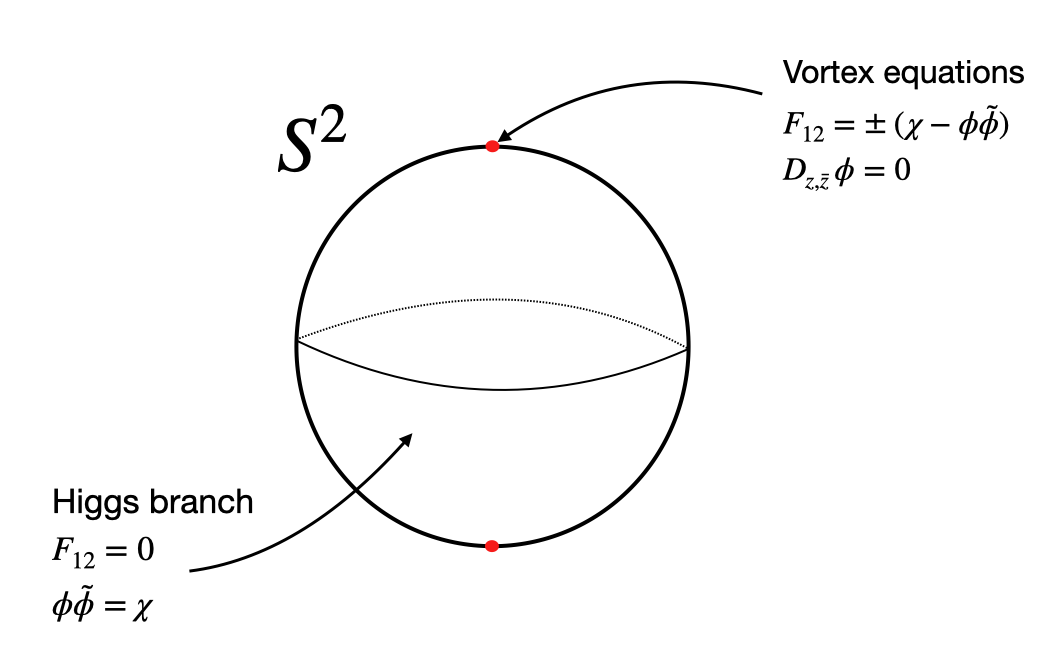
\includegraphics[width=.7\textwidth]{sol.png}
\end{figure}
The solution to the vortex equations are known to be instantons in $2d$. And now when we localize we have a finite sum on the Higgs branches. 

\section{Higgs branch localization}
New we will study what is called Higgs Branch Localization. Before we added a new $Q$-exact term that was not positive definite but by using $D$-term equations we could make it positive definite which was like changing the integration contour. We had two different solutions for the BSP equations on the sphere in the limit
\begin{equation}
	\underset{Q-\text{exact}}{\chi}\rightarrow\infty
\end{equation}
which is a ``fake'' parameter. \\
The moduli space of solutions of the vortex equations is separated into disconnected branches and each branch is characterized by a number: the vortex (or instanton) number. If we take $U(N)$ for example 
\begin{equation}
	k = \frac{1}{2\pi}\int_{\mathbb{R}^{2}}F \in \mathbb{Z}
\end{equation}
So the final form of the formula will be
\begin{equation}
\begin{split}
	\mathcal{Z}_{S^{2}} = \sum_{\substack{\text{Higgs}\\ \text{Branch}\\ \text{(Finite)}}}e^{S_{cl}}\mathcal{Z}^{\prime}_{1-\text{loop}}\mathcal{Z}_{\text{vortex}}(q)Z_{\overline{\text{vortex}}}(\overline{q})
\end{split}
\end{equation}
where the $1$-loop determinant is similar to the last one. The interesting part are the other pieces: the vortex part comes out to be like the one for a theory in an $\Omega$-background since the poles are not flat, there is some residual curvature. This theory gives us a background potential which traps the vortices in the origin which makes the moduli space somewhat compact since the vortices cannot move to infinity
\begin{equation}
	\mathcal{Z}_{\text{vortex}}(q) = \sum_{k\ge 0}q^{k}\int_{\mathcal{M}_{k,\text{vortex}}}\dd{\text{Vol}}_{equiv},\qquad q=e^{-4\pi\xi-i\theta}
\end{equation}
What about the $\mathcal{M}_{k,vortex}$ moduli space? It is Kähaler and symplectic. In particular there is a closed symplectic $2$-form $\omega$ which gives us the volume through the $\mathrm{d}\omega$. In particular $\dd{\text{Vol}} = \omega^{l}/l!$ which in particular is infinite. In fact we want to evaluate the equivariant volume. First of all we have rotations of $\mathbb{R}^{2}$ and moreover we have flavour rotations of $\phi$. The first is abelian, in the second we take the maximal torus (we do equivariant cohomology on the maximal torus). For each of this we have to introduce a vector field $V$ (which is very general for now). The volume form is equivariant under the action of $V$ ${L}_{V} \omega=0$ however is not equivatiantly closed. We construct the equivatiantly closed form $\dd{\text{Vol}} = \exp\qty(\omega+\mu)$ where $\mu$ is the moment map for the $U(1)^{\#}$ action where $\dd{\mu} = \iota_{V}\omega$. One can show that this is equivatiantly closed.\\
What we would like to compute is (using a physicist way)
\begin{equation}
	\int_{\mathcal{M}_{k,\text{vortex}}}\dd{\text{Vol}}_{equiv} = 0d \text{ path integral of a theory that has } \mathcal{M}_{k,vortex} \text{ as its moduli space}
\end{equation}
This is called ADHM construction. The point is finding what this theory is. Let us consider a specific example: $2d$ $\mathcal{N}=(2,2)$ $U(N)$ SQCD with $N_{f}$ fundamentals and $\tilde{N}_{f}$ antifundamental with $N_{f},\tilde{N}_{f}>N$ and a FI $\xi>0$. We want to understand the vortex moduli space of this theory which was done by Hanany and Tong in 2003. We go to the $k$-vortex sector which is a $0d$ theory (dimensional reduction of $2d$ $\mathcal{N}=(0,2)$ which has the following ingredients: $U(k)$ vector $(\phi,\lambda,\bar{\lambda},D)$, one adjoint chiral $X,\chi$, $N$ fundamental chirals $I,\mu$, $N_{f}-N$ antifundamental chirals $J,\nu$ and $\tilde{N}_{f}$ fundamental Fermi multiplet $\xi, G$ (fermion and auxiliary scalar). To compute the equivariant volume we have to do the path integral of this theory which is a matrix model and is simple. Again we can use localization on this theory which is much more simple than the initial integral.\\
Essentially we have to compute the $1$-loop determinants
\begin{equation}
	\text{Chiral}\longrightarrow\int\dd{X}\dd{X}^{\dagger}\dd{\chi}\dd{\chi}^{\dagger}e^{-X^{\dagger}\phi^{2}X-\chi^{\dagger}\phi\chi}\sim \frac{1}{\phi}
\end{equation}
which by the example we can see that they are very easy. The result at the end is
\begin{equation}
	\mathcal{Z}_{k}=\oint_{C}\prod_{I=1}^{k}\frac{\dd{\phi}_{I}}{2\pi i} \mathcal{Z}_{vec}(\phi)\mathcal{Z}_{chiral}(M,\phi)\mathcal{Z}_{fermi}(\tilde{M},\phi)
\end{equation}
the contour is called Jeffry-Kirwan residue. By computing this residues 
\begin{equation}
	\mathcal{Z}_{vortex}^{SQCD} = \sum_{\vec{k}}\frac{q^{\abs{\vec{k}}}}{\vec{k}!}\frac{\prod_{i=1}^{N}\prod_{a=1}^{\tilde{N}_{f}}\qty(\frac{1}{\epsilon}\qty(M_{p_{i}}+\tilde{M}_{a}))_{k_{i}}}{\prod_{i\neq j}^{N}\qty(\frac{1}{\epsilon}\qty(M_{p_{i}}-M_{p_{j}})-k_{j})_{k_{i}}\prod_{i=1}^{N}\prod_{f\not\in 2\pi_{i}\xi}^{N_{f}}\qty(\frac{1}{\epsilon}\qty(M_{p_{i}}-M_{f})-k_{i})_{k_{i}}}
\end{equation}
in which the $k_{i}$ down are called Pockhammer symbols.\\

Let us remain on $2d$ $\mathcal{N}=(2,2)$ theories but now let's take a $T^{2}$ background. What is the object that we are computing? What are the observables that we can access? This is the superconformal index (elliptic genus)
\begin{equation}
	\mathcal{I}(\tau,z,\nu_{\alpha}) = \Tr_{RR}(-1)^{F}q^{H_{L}}\bar{q}^{H_{R}}y^{J_{L}}\prod_{a}\xi^{k_{a}},\qquad q=e^{2\pi i\tau},y=e^{2\pi i z},\xi_{a}=e^{2\pi i \nu_{a}}
\end{equation}
This object does not actually depend on $\bar{q}$, only states with $H_{R}$, the right-movint hamiltonian, contribute. We can send $y\rightarrow 1$ which reduces this to the Witten index since even the dependence on $q$ drops.\\
When we go to euclidean, we compactify time and since the theory is on a cylinder, it becomes a torus in euclidean and this partition function counts the number of states.
